%! Author = nadutkinfedor
%! Date = 09.01.2024

% Preamble
\documentclass[11pt]{article}
\usepackage[left=2cm, right=1cm, top=2cm, bottom=2cm, bindingoffset=0cm]{geometry}

% Packages
\usepackage[utf8]{inputenc}
\usepackage[russian]{babel}
\usepackage{amsmath}
\usepackage{hyperref}
\usepackage{graphicx}
\usepackage{misccorr}
\usepackage{listings}
\usepackage{xcolor}
\usepackage{titlesec}
\usepackage{minted}
\usepackage{color}
\usepackage{enumitem}
\usepackage{indentfirst}

%listing settings
\definecolor{dkgreen}{rgb}{0,0.6,0}
\definecolor{gray}{rgb}{0.5,0.5,0.5}
\definecolor{mauve}{rgb}{0.58,0,0.82}

\lstset{language=SQL,
    basicstyle={\small\ttfamily},
    belowskip=3mm,
    breakatwhitespace=true,
    breaklines=true,
    classoffset=0,
    columns=flexible,
    commentstyle=\color{dkgreen},
    framexleftmargin=0.25em,
    keywordstyle=\color{blue},
    numbers=none, %If you want line numbers, set `numbers=left`
    numberstyle=\tiny\color{gray},
    showstringspaces=false,
    stringstyle=\color{mauve},
    tabsize=3,
    xleftmargin =1em,
    backgroundcolor=\color{gray!10}
}

\lstset{ %
    backgroundcolor=\color{white},   % choose the background color
    basicstyle=\footnotesize,        % size of fonts used for the code
    breaklines=true,                 % automatic line breaking only at whitespace
    captionpos=b,                    % sets the caption-position to bottom
    commentstyle=\color{dkgreen},    % comment style
    escapeinside={\%*}{*},          % if you want to add LaTeX within your code
    keywordstyle=\color{blue},       % keyword style
    stringstyle=\color{mauve},     % string literal style
}

% link setting
\hypersetup{
    colorlinks=true,
    linkcolor=blue,    % Синий цвет для внутренних ссылок
    filecolor=magenta, % Можно выбрать другой цвет для файлов
    urlcolor=blue      % Синий цвет для URL
}

% Title
\title{DB internals. Третья лекция}
\author{Надуткин Федор }
\date{February 2024}

\titleformat{\section}[block]{\Huge\bfseries\filcenter}{}{1em}{}
\titleformat{\subsection}[block]{\LARGE\bfseries\filcenter}{}{1em}{}
\titleformat{\subsubsection}[block]{\Large\bfseries\filcenter}{}{1em}{}

% Document
\begin{document}

    \maketitle
    \newpage

    \section*{Ключевые оптимизации}

    \begin{itemize}
        \item \textbf{Нормализация} --- приведение плана к каноническому виду, которы позволяет применить наибольшее количество оптимизаций.
        \item \textbf{Оптимизация} --- Уменьшение количество вычислений.
        Нахождение более дешёвых планов.
    \end{itemize}

    На практике, в обычных движках нормализации и оптимизации чередуются подряд.
    Зачастую они бывают узко специализированными, поэтому <<прийти и посмотреть как это сделано>> не получится, нужно выделять паттерны.

    \subsection*{Нормализация и упрощение выражений}

    \begin{figure}[h!]
        \centering
        \includegraphics*[width=0.7\textwidth]{Pictures/Ключевые оптимизации/Нормализация и упрощение выражений}
        \caption{Нормализация и упрощение выражений}
    \end{figure}

    \textbf{Плюсы:}
    \begin{itemize}[label=+]
        \item Отсутствие последующего пересчёта на следующих этапах.
        \item Упрощение анализа.
        Например, становится легче искать похожие подпланы.
        Мы привели выражение в нормальную форму.
    \end{itemize}

    \textbf{Минусы:}
    \begin{itemize}[label=-]
        \item Необходимы подключение интерпретаторов, оптимизаторов, калькуляторов \dots, что сильно усложняет структуру и может сделать проигрыш в некоторых ситуациях.
        \item Требуют дополнительной логики и алгоритмов.
    \end{itemize}

    \newpage

    \subsection{Filter into Join}

    \begin{figure}[h!]
        \centering
        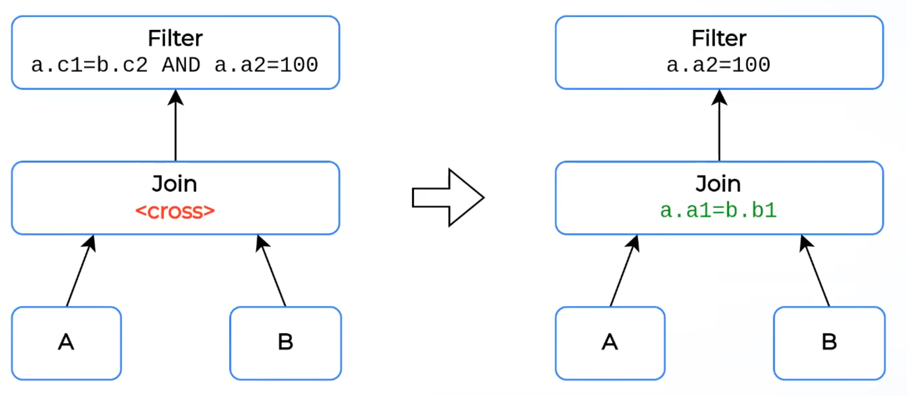
\includegraphics[width=0.7\textwidth]{Pictures/Ключевые оптимизации/Filter into Join}
        \caption{Filter into Join}
    \end{figure}

    \subsection{OuterJoin to InnerJoin}

    \begin{figure}[h!]
        \centering
        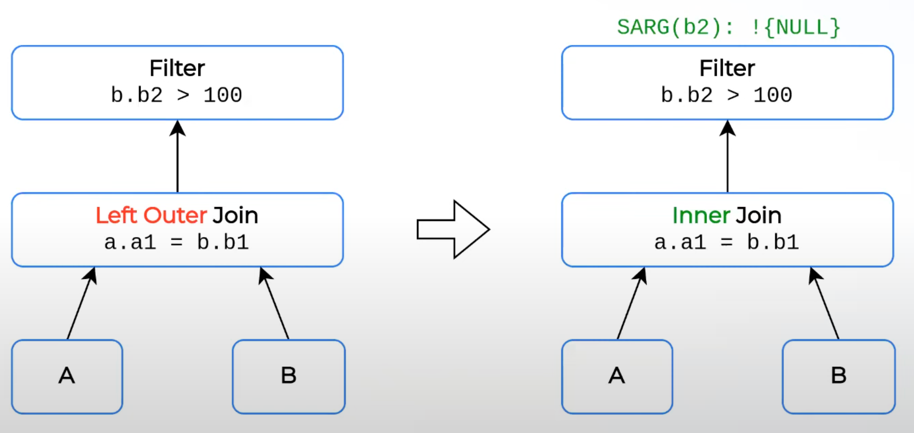
\includegraphics[width=0.7\textwidth]{Pictures/Ключевые оптимизации/OuterJoin to InnerJoin}
        \caption{OuterJoin to InnerJoin}
    \end{figure}

    В случае, если для левого ключа нет колонки справа (и наоборот) \texttt{OuterJoin} заменяет правый ключ на \texttt{NULL}.
    Если в будущем у нас будут операторы, которые отбрасывают такие ключи, то можно заменить \texttt{OuterJoin} на \texttt{InnerJoin}.

    \subsection*{Упрощение агрегатов}

    Иногда данные в таблице у нас разрозненные, а как следствие агрегаторы по значению будут лишь возвращать значение по ключу.
    Такие операторы можно (и нужно) заменить или выбросить.

    \newpage

    \subsection{Одни операторы, через другие}

    Некоторые движки могут не поддерживать непосредственно какие-то операции, но хорошо поддерживают другие.
    Мы можем попробовать выразить один оператор через другие.
    Например, \texttt{Distinct Aggregate} через \texttt{Join}.

    \begin{figure}[h!]
        \centering
        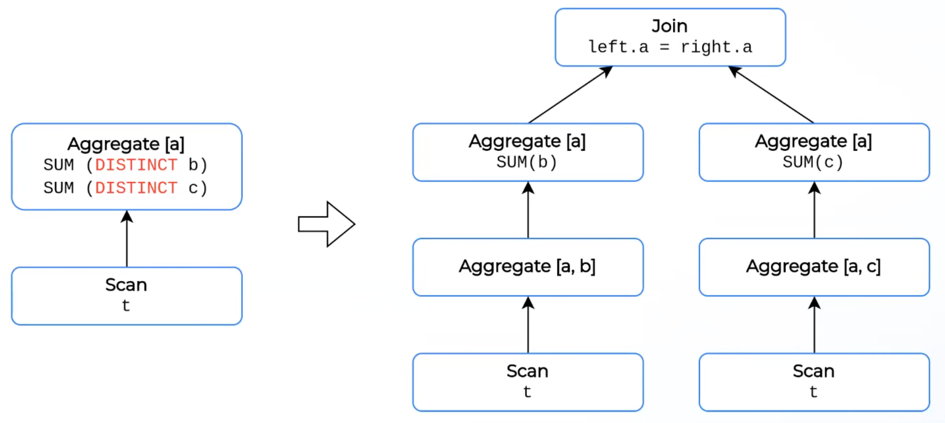
\includegraphics[width=0.7\textwidth]{Pictures/Ключевые оптимизации/Distinct Aggregate to Join}
        \caption{Distinct Aggregate to Join}
    \end{figure}

    Или например \texttt{Intersect}, \texttt{Minus}, \dots выразить через \texttt{UnionAll}.
    Или например \texttt{Intersect}, \texttt{Minus}, \dots выразить через \texttt{UnionAll}.

    \begin{figure}[h!]
        \centering
        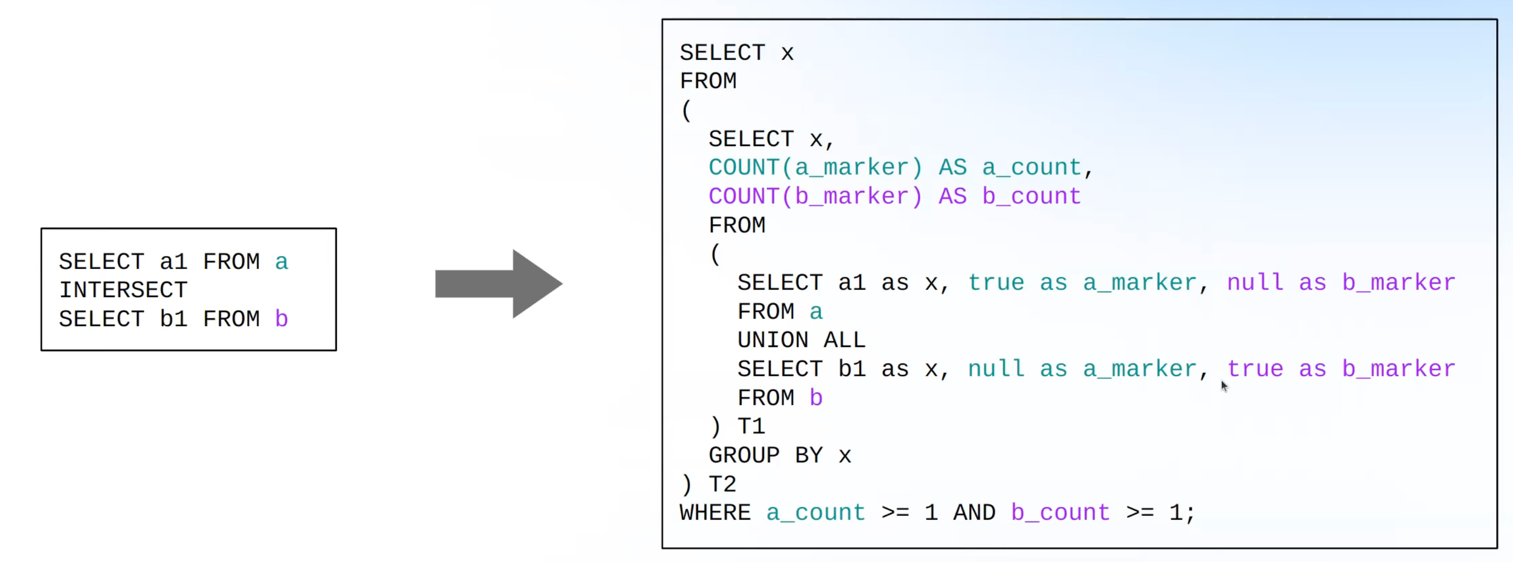
\includegraphics[width=\textwidth]{Pictures/Ключевые оптимизации/Intersect из UnionAll}
        \caption{Intersect из UnionAll}
    \end{figure}

    \newpage

    \subsection{Переписывание подзапросов}

    Поддерживание коррелированных подзапросов достаточно трудная задача, более того в распределённых системах она только вредит, как следствие можно переделать запрос на запрос без корреляций.

    \href{https://cs.emis.de/LNI/Proceedings/Proceedings241/383.pdf}{Доказательство, что из любого коррелированного запроса можно сделать некоррелированный}.

    \href{https://alibaba-cloud.medium.com/query-optimization-technology-for-correlated-subqueries-8d265a51f58e}{Хороший пример как делают в Алибабе (читать под ВПН)}.

    На практике от коррелированных подзапросов не избавляются полностью, но стараются.

    \begin{figure}[h!]
        \centering
        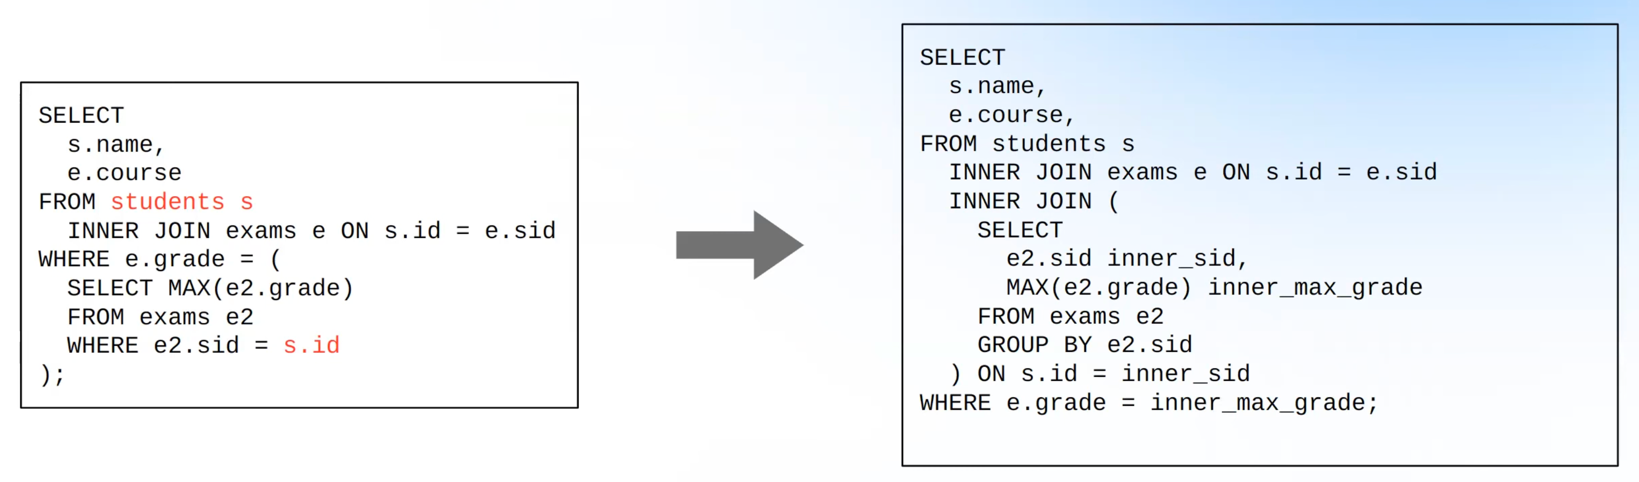
\includegraphics[width=\textwidth]{Pictures/Ключевые оптимизации/Переписывание подзапросов}
        \caption{Переписывание запроса с корреляцией на запрос без неё}
    \end{figure}

    \subsection{Filter pushdown}

    \begin{figure}[h!]
        \centering
        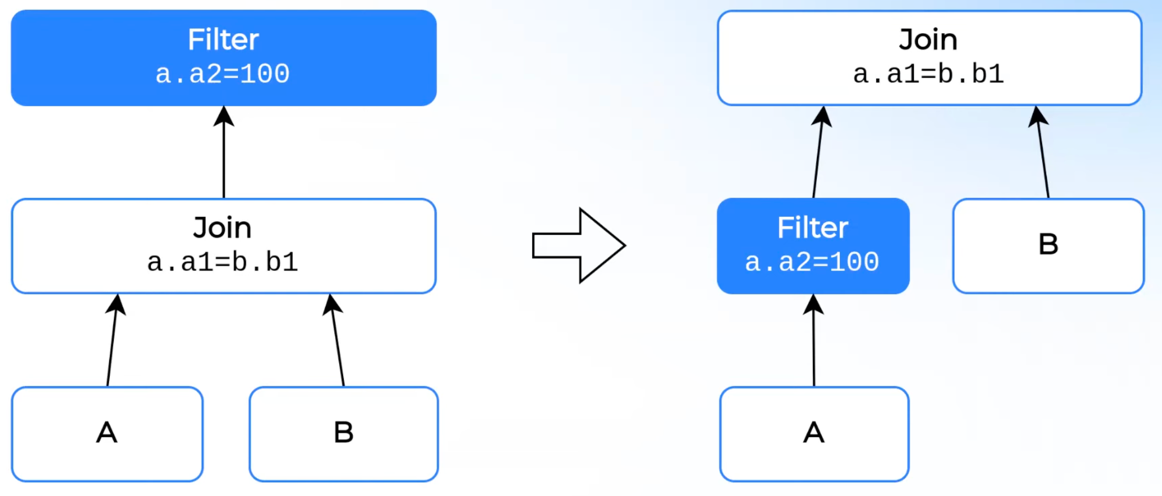
\includegraphics[width=\textwidth]{Pictures/Ключевые оптимизации/Filter pushdown}
        \caption{Filter pushdown}
    \end{figure}

    \texttt{Filter} можно прокинуть практически через любой оператор, а значит опустить его всегда можно.
    Однако, если \texttt{Filter} не всегда хорошо фильтрует, то pushdown может и навредить.

    \subsection{Filter pull up}

    \begin{figure}[h!]
        \centering
        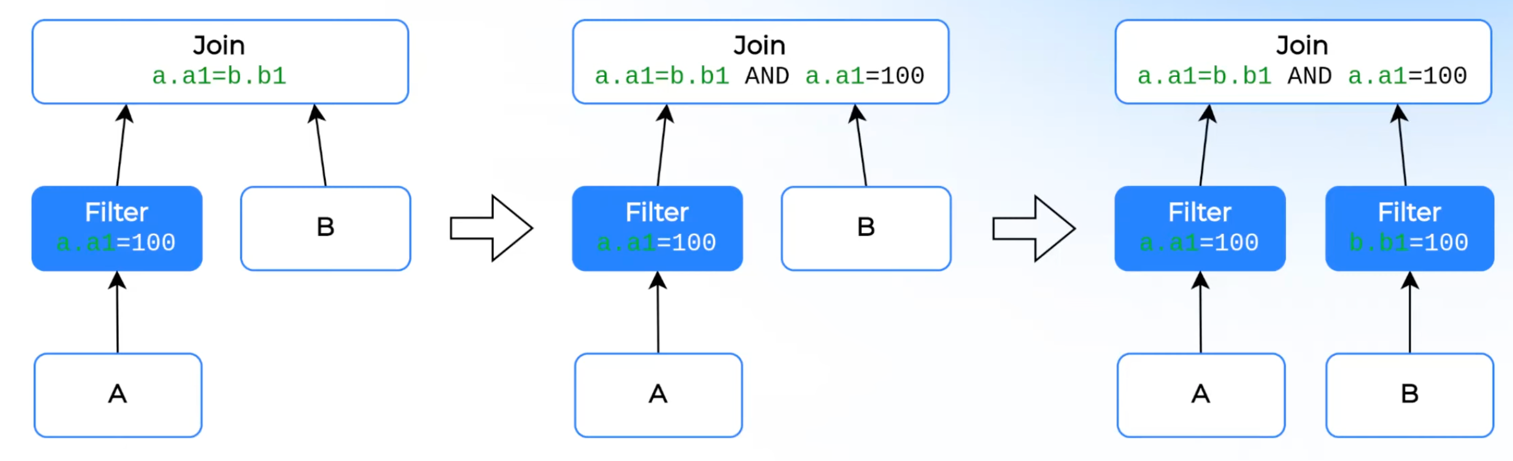
\includegraphics[width=\textwidth]{Pictures/Ключевые оптимизации/Filter pull up}
        \caption{Filter pull up}
    \end{figure}

    Перемещение фильтра наверх иногда позволяет создать дополнительные транзитивные предикаты.

    \subsection{Dynamic/Runtime Filters}

    \begin{figure}[h!]
        \centering
        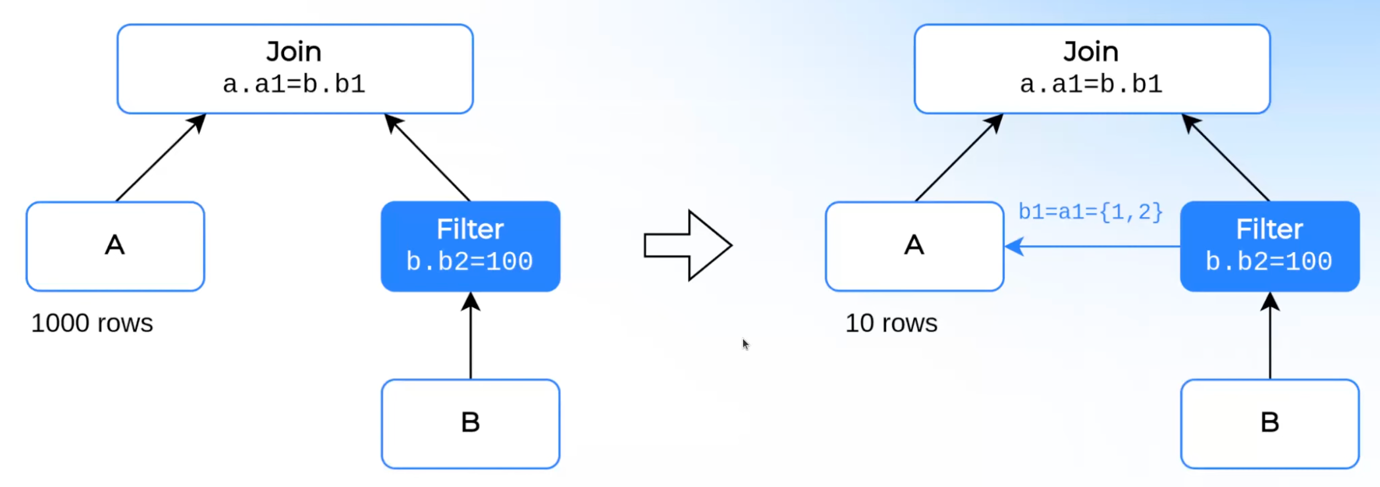
\includegraphics[width=\textwidth]{Pictures/Ключевые оптимизации/Dynamic filters}
        \caption{Dynamic Filters}
    \end{figure}

    Можно посмотреть какие значения $b_1$ соответствуют $b_2 = 100$, если там будет мало различных значений, то мы получим дополнительный фильтр.

    \subsection{Pushdown других операторов}

    \begin{itemize}
        \item \textbf{Project} --- передача меньшего количества атрибутов между операторами.
        \item \textbf{Aggregate} -- уменьшение количества кортежей как можно раньше.
        \item \textbf{Limit} --- ограничить набор данных, возвращаемых нижестоящим оператором.
    \end{itemize}

    \subsection{Spool}

    Поиск повторяющихся операторов.

    \begin{figure}[h!]
        \centering
        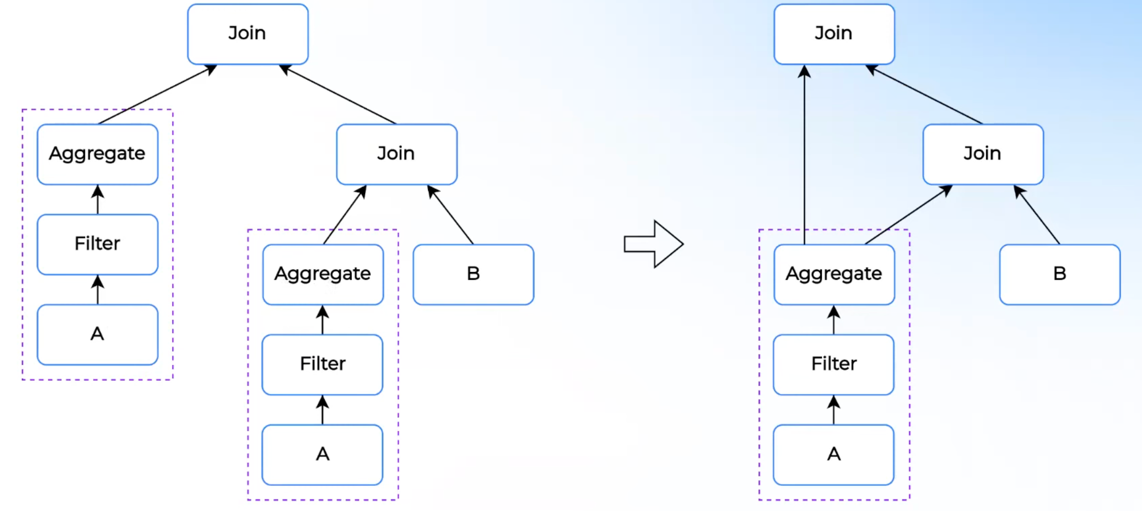
\includegraphics[width=0.8\textwidth]{Pictures/Ключевые оптимизации/Spool}
        \caption{Spool}
    \end{figure}

    Приводим дерево к ациклическому графу \textbf{DAG}, таким образом мы можем избежать выполнения идентичных подпланов.

    \begin{itemize}[label=-]
        \item Может ухудшиться из-за снижения параллелизма.
        \item Риски \texttt{Deadlock}, так как оба оператора смотрят в одну и ту же область и могут её забивать и блокировать друг друга.
    \end{itemize}

    \subsection{Materialized views}

    \begin{figure}[h!]
        \centering
        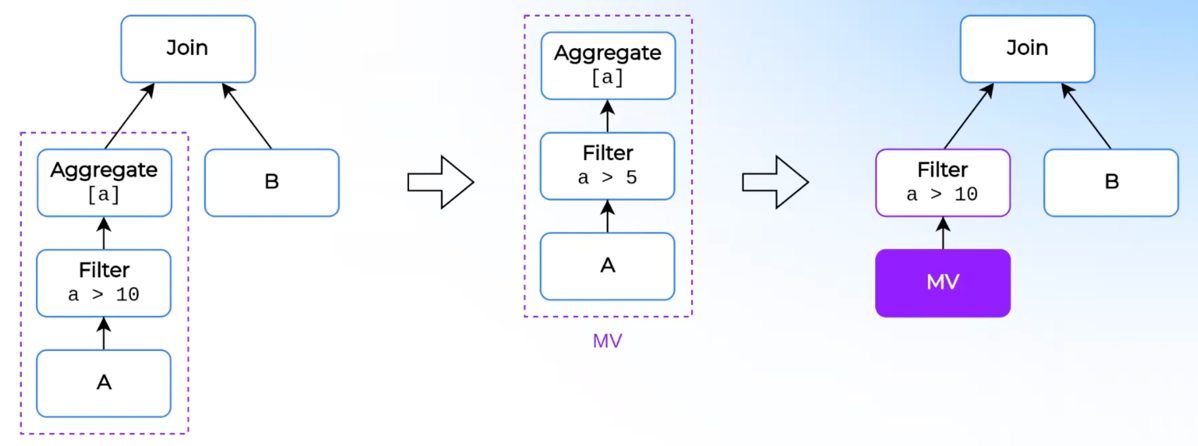
\includegraphics[width=\textwidth]{Pictures/Ключевые оптимизации/Materialized views}
        \caption{Materialized views}
    \end{figure}

    Имея набор \texttt{Materialized views} мы можем сократить нагрузку на вычисления, однако это потребляет дополнительную память.
    \begin{itemize}
        \item Как подобрать оптимальный набор для заданной нагрузки?
        \item Как поддерево в плане переписать на \texttt{materialized view}?
    \end{itemize}

    \textbf{Для решения этого есть: }
    \begin{itemize}
        \item \href{https://dl.acm.org/doi/10.1145/235968.233333}{Базовый алгоритм}
        \item \href{https://www.researchgate.net/publication/220895475_Efficient_Utilization_of_Materialized_Views_in_a_Data_Warehouse}{Пример алгоритма}.
    \end{itemize}
\end{document}